\section{Benchmarks}
\begin{frame}
    \frametitle{CLIP vs ResNet-50}
    \begin{columns}[T]
        \begin{column}{0.35\textwidth}
            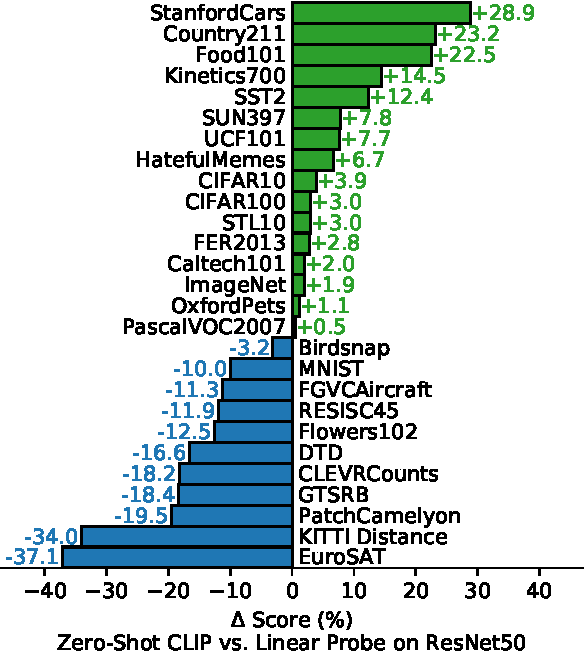
\includegraphics[width=\textwidth]{./images/zs-clip-vs-rn50}\framecite{clip}
        \end{column}
        \pause
        \begin{column}{0.65\textwidth}
            \textbf{Wins}: 16 datasets
            \begin{itemize}
                \item Broad, "general" classes
                \item Datasets with little labeled data
            \end{itemize}

            \pause

            \textbf{Losses}: 11 datasets
            \begin{itemize}
                \item Spezialized classes
                \item Abstract tasks
                \item Counting
                \item Self-driving tasks
            \end{itemize}
        \end{column}
    \end{columns}
\end{frame}

\begin{frame}
    \frametitle{Optimizations}
    \scriptsize
    \begin{columns}[T]
        \begin{column}{0.65\textwidth}
            \textbf{Prompt engineering}
            \begin{itemize}
                \item Provide context: "A photo of a \{ label \}, a type of \{ class \}"
                \item For OCR: Put quotes around the prompt
                \item For sattelite images: "A sattelite photo of a \{ label \}"
                \item Can be further optimized with Context Optimization \framecite{Zhou2021LearningTP}
            \end{itemize}

            \pause
            \vspace{1em}

            \textbf{Ensembling}
            \begin{itemize}
                \item Average over encodings of multiple similar prompts for the same category
                \item Improve performance by 3.5\%
            \end{itemize}
            \vspace{1em}

            Prompt engineering and ensembling improve performance by 5\%
        \end{column}
        \pause
        \begin{column}{0.35\textwidth}
            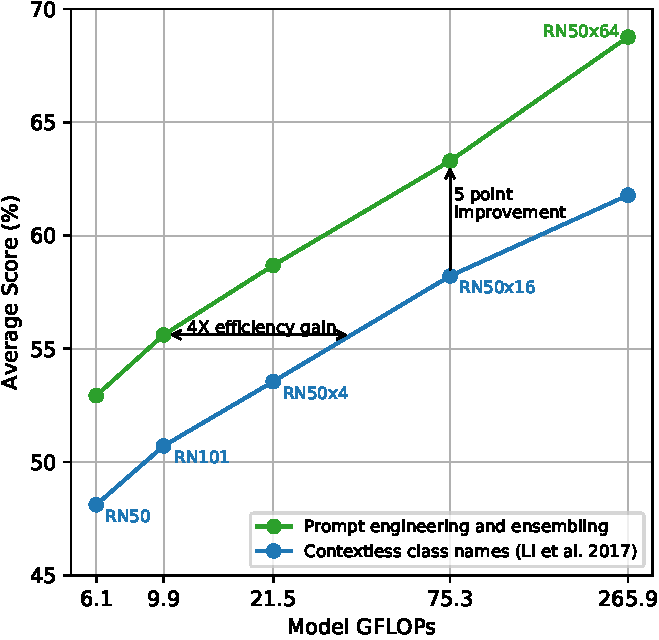
\includegraphics[width=\textwidth]{./images/prompt-engineering}\framecite{clip}
        \end{column}
    \end{columns}
\end{frame}
